This paragraph will present the two dashboards implemented, the design principles used, and the SA demons that were tried to avoid. As mentioned before, to ensure that most of the requirements identified in the previous stage could be represented, it was decided to use a dataset entirely created by us to have full control over the data and its structure.

The whole system is divided into two dashboards, each associated with multiple goals. The first dashboard aims to establish \textbf{Common Operational Picture} that allows students to have an understanding of the current situation by integrating multiple subgoals into coherent visualizations. 
Unlike, the second dashboard, focuses on tracking and presenting student learning progress within a specific course.

\begin{itemize}
    \item \textbf{Dashboard I}: Subgoal 1.2.1 - Improve student engagement with the platform and Subgoal 1.2.2 - Optimize student learning through personalization.
    \item \textbf{Dashboard II}: Subgoal 1.1.1 - Comprehension of the fundamental concepts of cybersecurity, Subgoal 1.2.1 - Improve student engagement with the platform and Subgoal 1.2.2 - Optimize student learning through personalization.
\end{itemize} 

Both of the dashboards attempt to achieve the trade-off between supporting the operator's goal and supporting the overall SA. By placing the most important information appropriately at the center of each dashboard and positioning the supporting information on the sides, we ensure that relevant data is easily accessible to the student. This design choice is intended to reduce the cognitive load on the student, so he/she can quickly understand his current situation and make informed decisions about his learning path.

Some common guidelines were used to blend the student experience and create a sense of confidence in switching between the different dashboards and to enhance efficiency by transporting the experience matured in one dashboard to the other. This is helpful so that the student can create expectations about the interface, increasing his or her satisfaction.

\section{Dashboard I}

The objectives of this dashboard are to maintain student engagement with the platform and to assist in tailoring the learning process to meet the student's needs.

To ensure the student is aware that he/she are on the home page of the platform, the name of the platform \textbf{OffSec} is included, representing \textit{Offensive Cybersecurity}. Additionally, a "Welcome Marta!" message is displayed to emphasize that this dashboard is the home page. These two elements help prevent the student from using an incorrect mental model when interpreting the dashboard's components, effectively avoiding the \textbf{Wrong Mental Model} demon.

\begin{figure}[H]
    \centering
    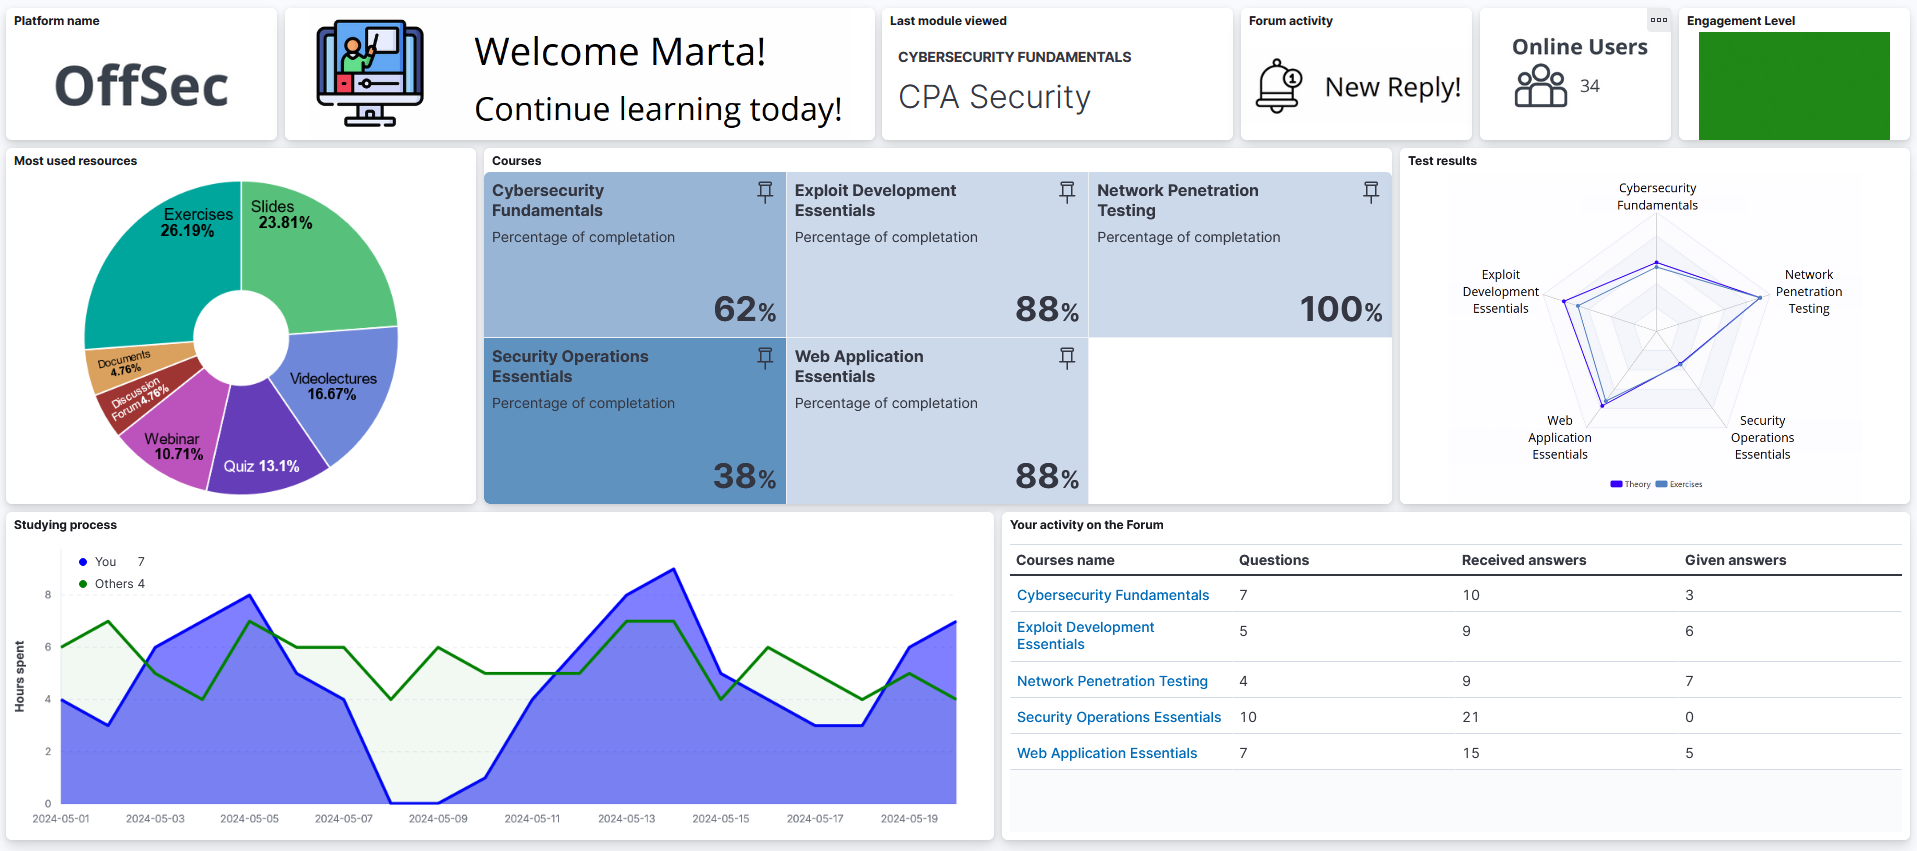
\includegraphics[width=0.9\textwidth]{assets/dashboard_1.png}
    \caption{Dashboard I}
    \label{fig:dashboard_1}
\end{figure}

To ensure compliance with \textbf{Design Principle 4} and in order to support \textbf{Design Principle 1}, the dashboard should be designed with central elements supporting specific goals, 
surrounded by elements that provide an overview of the student's progress. But typically, e-learning systems display an overview of the courses the student is following. 
Therefore, we adopted this common approach for our system as well.
As shown in Figure 6.1, the center of the screen features a matrix of the various courses the student needs to complete for upskilling, 
with each course's completion percentage clearly indicated. This allows students to quickly understand his/her progress, supporting his/her 
overall SA.

This design choice supports both \textbf{Design Principle 5 and Design Principle 6} through the effective use of salience. 
Darker colors in the matrix highlights courses with lower completion percentages, drawing the student's attention to these areas and guiding the student towards the courses that need more
attention before his/her deadlines. This can prompt a shift from data-driven to goal-driven behavior, encouraging the student to prioritize completing the less finished courses. 

In order to form the right Global SA of the student, on 
the right side of the screen there is a spider chart showing the results of the student on theoretical tests and
practical tests, weighted on the number of tests completed for the course.
Instead, on the left side of the screen, there is a
donut chart, that shows which resources the student has preferred for the different courses 
the student has used, in order to support the \textbf{Subgoal 1.2.2}.

The linear graph, which shows the student's time spent on the platform since the start of the upskilling process, supports \textbf{Subgoal 1.2.1}. 
It allows the student to compare his/her time spent on the platform with the time spent by other students. 
By observing this graph, the student can become aware of his/her own hours invested. 
If the student notices that other students have spent significantly more time on the platform, it can serve as a motivation for him/her to dedicate more time to the learning process. 
This comparative visualization encourages students to increase his/her engagement and commitment to the platform, cultivating a more competitive and driven learning environment.


\begin{figure}[H]
    \centering
    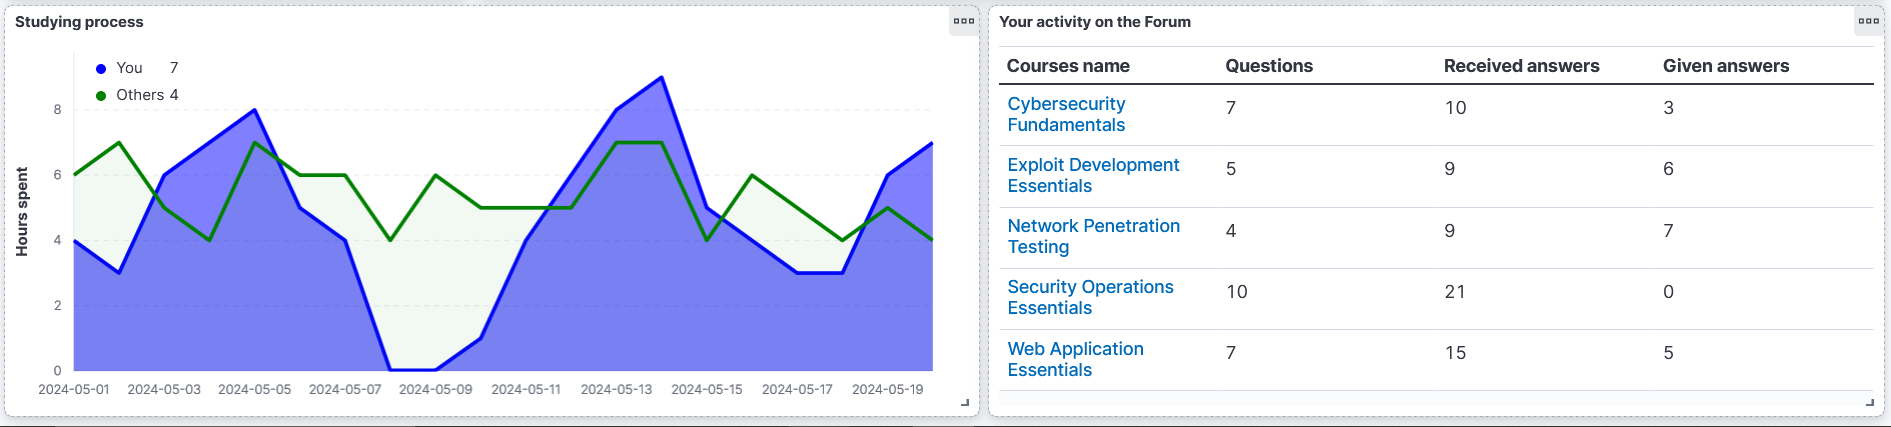
\includegraphics[width=0.9\textwidth]{assets/dashboard_1_121.png}
    \caption{Dashboard I - Subgoal 1.2.1}
    \label{fig:dashboard_1_subgoal_121}
\end{figure}

The elements present in Figure 6.3 indicate student engagement with the platform, presenting (from right to left) the computed engagement level using the CST described in a previous chapter, the number of students currently online, a notifications section from the forum, and an element displaying the last viewed module. Together, these components maintain continuous global situational awareness to prevent the occurrence of the \textbf{Attentional Tunneling} demon.
In particular, the last viewed module element helps to avoid the \textbf{Memory Trap} demon by providing a quick reminder of the student's most recent activity, reducing the cognitive load associated with remembering the last module he/she accessed.

\begin{figure}[H]
    \centering
    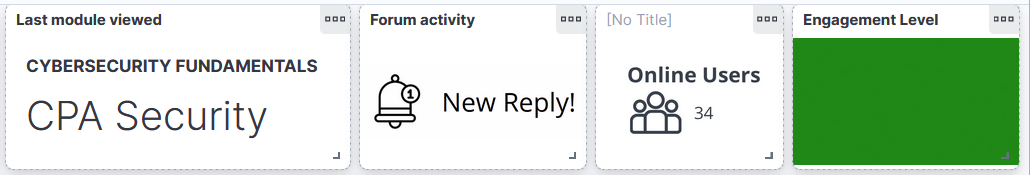
\includegraphics[width=0.9\textwidth]{assets/dashboard_1_globaltop.png}
    \caption{Dashboard I - Global Top}
    \label{fig:dashboard_1_global_top}
\end{figure}

Given that human attention and working memory are limited, most of the information has been processed and integrated in terms of Level 2 SA, supporting comprehension. Therefore, \textbf{Design Principle 2} has been satisfied.
This allowed us to avoid the \textbf{Memory Trap} demon, which can occur when students are required to remember too much information. 
Moreover, the use of visualizations such as the spider chart and the donut chart helps to avoid the \textbf{Data Overload} demon and the \textbf{Complexity Creep} demon, as he/she provide a more compact representation of the data, reducing the amount of information that needs to be processed.

Another element that could contribute to support the \textbf{Design Principle 5} is the presence of the notifications from the forum, which can capture the student's attention and facilitate the switch between goal-driven and data-driven processing. This element helps to avoid the \textbf{Attentional Tunneling} demon.

The engagement level element is displayed as a square shape filled with a color, which can capture the student's attention when it is not needed, causing a bit of the \textbf{Misplaced Salience} demon. 
Though, the use of colors (green, yellow, orange) suggests that if the indicator is green, the student's attention may briefly focus on it, indicating satisfaction or a certain level of confidence in his/her engagement level. Unlike the yellow and orange colors that might encourage the student to spend more time on the platform and interact more actively with it.

The dashboard effectively prevents the \textbf{Out of the Loop} demon since there are no autonomous functions that operate independently and since it is crucial for the student to make decisions about his/her actions and timing autonomously.

Our goal is also to fulfill \textbf{Design Principle 3}, which emphasizes providing Level 3 assistance. 
This is facilitated within our dashboard through the inclusion of a forum. By interacting with other students to discuss course-related 
questions and challenges, students can obtain answers and support. This interaction could encourage them to continue his/her learning journey, 
thereby reducing the likelihood of abandoning the platform. 

\section{Dashboard II}

The goal of the dashboard is to support the student's learning process within a specific course. It is characterized by a title \textbf{Cybersecurity Fundamentals} to indicate the course the student is currently focusing on. The inclusion of a specific course title on the dashboard plays a crucial role in preventing student confusion, especially given the variety of courses a student might be enrolled in. 
In this way, it mitigates the risk of the \textbf{Wrong Mental Model} demon, ensuring that students maintain an accurate understanding of his/her learning progress and requirements within the context of the specific course he/she are viewing. 

The choice of different data visualizations used made it possible to reduce the effects of the \textbf{Data Overload} demon as well, by being able to convey the information by expressing it in graphical form rather than in textual or tabular form (e.g., pie charts for the most used resources), reducing the cognitive load on the student. 

A first view of the second dashboard is shown in the following figure.

\begin{figure}[H]
    \centering
    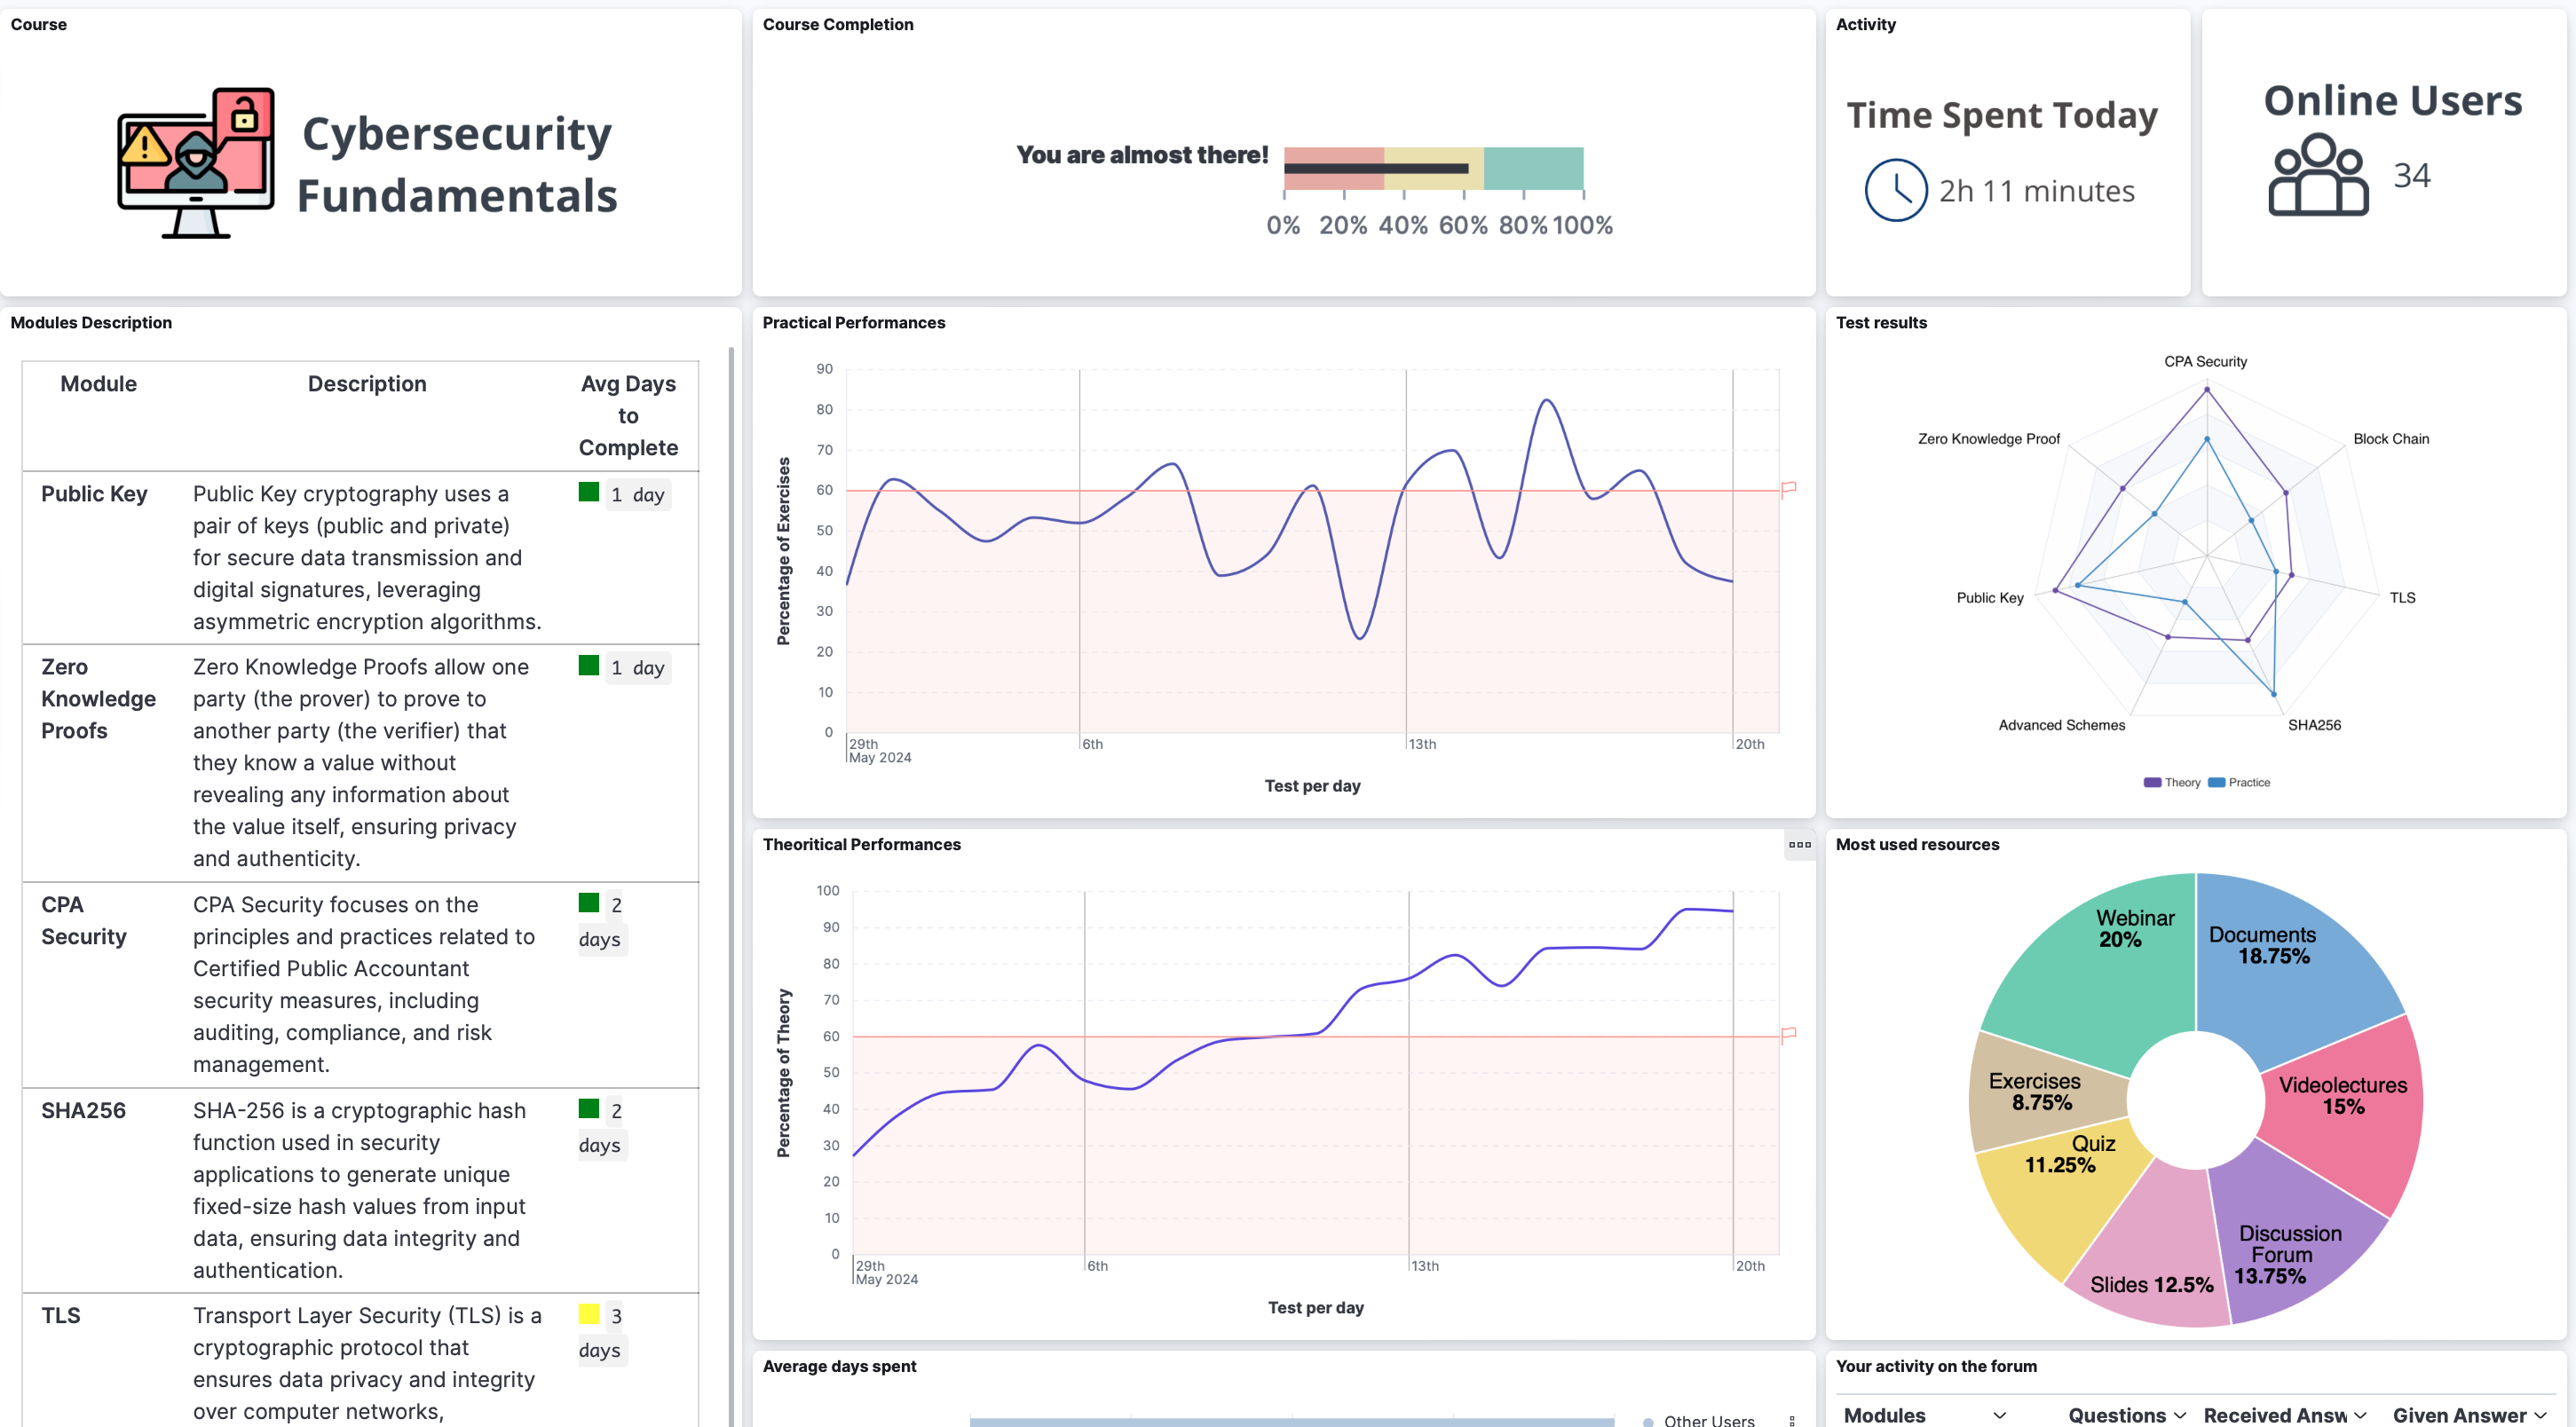
\includegraphics[width=0.9\textwidth]{assets/dashboard_2.png}
    \caption{Dashboard II}
    \label{fig:dashboard_2}
\end{figure}

With multiple subgoals active on the dashboard, it’s important that when a student opens it, he/she can quickly figure out the necessary information to achieve his/her objectives. 

This follows \textbf{Design Principle 1}, which ensures that information is provided effectively to support decision-making. When a student clicks on a course, he/she will see two line charts in the center of the dashboard showing his/her progress and the course completion status.

These charts, like the others on the dashboard, also satisfy \textbf{Design Principle 2} because the interface provides already processed and integrated information at Level 2. Specifically, the Level 2 and Level 1 data allow for a complete understanding of the situation, such as the student's performances in the course, without the need for further processing.

To ensure that salience is appropriately balanced within the dashboard, the latter is placed only on information considered important. For instance, the red threshold line in the main charts indicates that if a student's end-of-module test scores fall below 60\%, he/she needs to decide on a strategy for improvement. Hence, this visual cue helps students understand that he/she should aim for scores above this threshold.

The two line charts, also support \textbf{Design Principle 3} by providing level 3 projection assistance. This means that if a student maintains consistent performance across multiple modules, it can be projected that he/she will likely perform well in future modules. 

\begin{figure}[H]
    \centering
    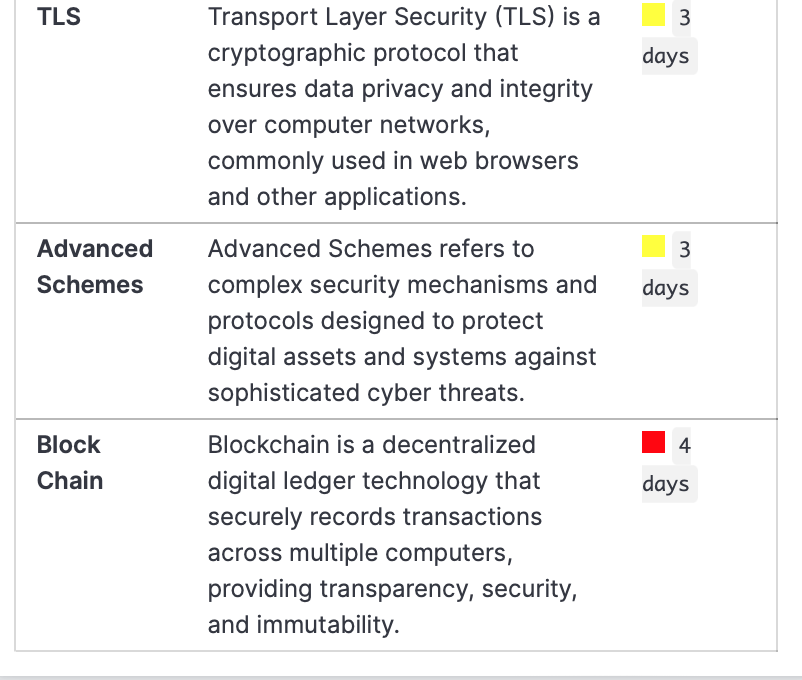
\includegraphics[width=0.3\textwidth]{assets/descriptionmodule.png}
    \caption{Dashboard II - Progress}
    \label{fig:dashboard_2} 
\end{figure}

As we can see in Figure 6.5, the estimated completion days for each module, within the section where the modules are listed with their description, are highlighted in red if they exceed four days, based on data from previous students who have taken the course. This alerts the student that it may be necessary to put in more effort for these particular modules.
The use of red to draw attention to critical areas complies with \textbf{Design Principle 6}, clearly signaling to the student where he/she needs to focus and prompting him/her to take corrective action if necessary.

The dashboard also includes a gauge chart dedicated to overall course completion. If a student has completed less than 40\% of the course, this chart will highlight the need for increased attention to ensure timely course completion.
The addition of a course completion chart helps reduce the cognitive load on the student by offering a visual depiction of his/her progress. This feature was intentionally introduced to prevent the student from having to remember the completion percentage shown on the main dashboard and to overcome relying on memory (facing the \textbf{Memory Trap} demon), which can often not guarantee accurate awareness and decision-making.

Given that the dashboard supports three subgoals, it is likely that when a student first opens the dashboard for a specific course, it will be done to check his/her progress. 

Through various charts—such as those showing the theoretical and practical test performance, course completion status, and average grades, he/she can assess the level of understanding of the course. 
These elements also supports the subgoal related to optimizing learning through personalization, including a pie chart that shows the usage of different learning materials for each module in order to show his/her learning preferences. 

\begin{figure}[H]
    \centering
    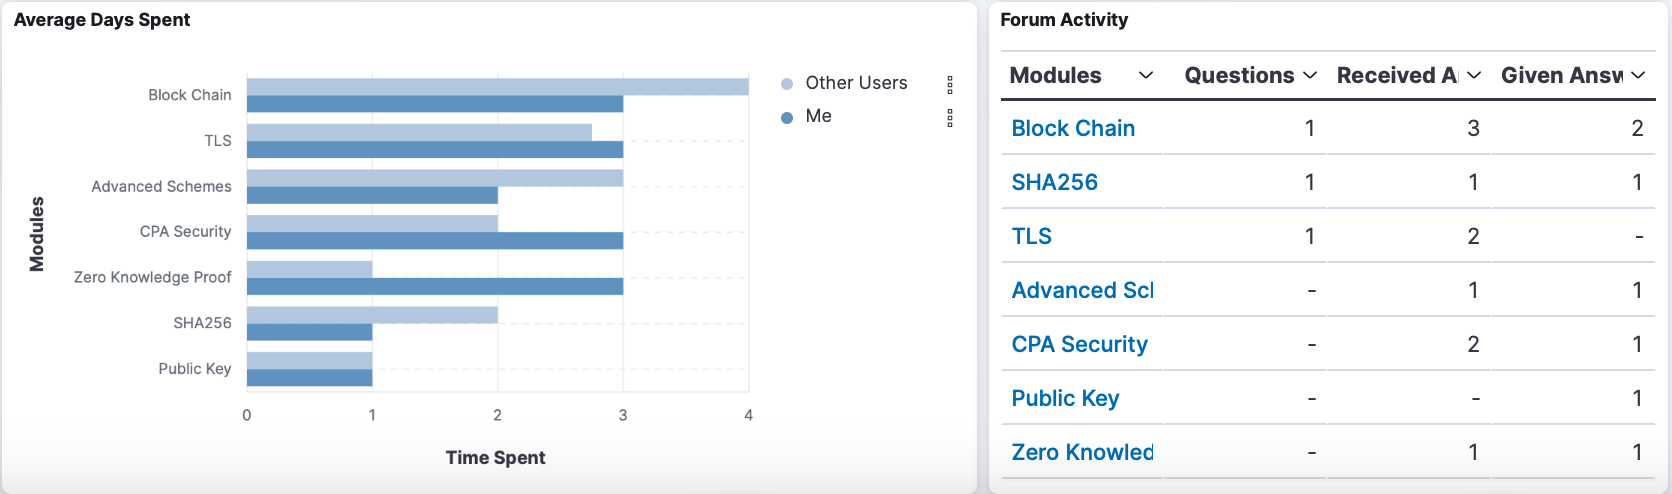
\includegraphics[width=0.9\textwidth]{assets/forum2.png}
    \caption{Dashboard II - Forum}
    \label{fig:dashboard_2}
\end{figure}

\begin{figure}[H]
    \centering
    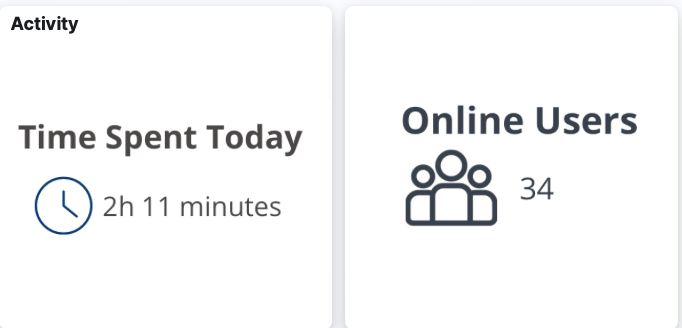
\includegraphics[width=0.3\textwidth]{assets/activity2.png}
    \caption{Dashboard II - Student Activity}
    \label{fig:dashboard_2}
\end{figure}

The elements in Figure 6.6 and 6.7 support goals related to engagement with the platform such as activities in the forum, the number of students online at the time of access, the time spent on the platform, and the days taken to complete each module compared to other students.

Therefore, we assume that at first glance, the student decides to focus on the first subgoal \textbf{Comprehension of the fundamental concepts of cybersecurity} to reach his/her objective and then potentially switches to other supported goals as he/she shifts the attention to the other charts. This approach could satisfy \textbf{Design Principle 5 and Design Principle 4} by including elements in the dashboard that capture attention on aspects satisfying different goals. This prevents attention from being confined to a limited set of information, thereby overcoming the issue of \textbf{Attentional Tunneling} demon and supporting the switch between goal-driven and data-driven modes based on the goal the student wishes to achieve.

